\documentclass[12pt]{article}

\usepackage{bm, graphicx, amssymb, amsmath, mathtools}
\usepackage[margin=1 in]{geometry}
\usepackage{mathtools}
\usepackage{epstopdf}
\usepackage{enumitem}
\usepackage{color}

\newcommand{\ds}{\displaystyle}
\newcommand{\B}[1]{{\bm #1}}
\newcommand{\U}[1]{{\hat{\bm #1}}}
\newcommand{\T}{^{\mbox{\tiny T}}}
\newcommand{\dd}{\; \text{d}}

%\thispagestyle{empty}

\begin{document}

\newif\ifsolution    % Declaration, defaults to false

%% Comment out this line to hide solutions
\solutiontrue

\begin{center}{\bf AERO-222: Introduction to Aerospace Computation - Fall 2021\\ Homework \#2 - Due Date: Wednesday, October 6, 2021} \vspace{0.5cm}

\textbf{\underline{Show all work and justify your answers!}} \vspace{0.5cm}
\end{center}

{\Large \textbf{Instructions}}
\begin{itemize}
	\item \textit{This homework contains both handwritten and coding problems and shall be submitted according to the following guidelines.}
	\item \textit{Hardcopy:}
	\begin{itemize}
	    \item \textit{Due on CANVAS at 11:59 PM on the day of the deadline.}
	    \item \textit{Shall include screenshots of any hand-written work.}
	    \item \textit{For coding problems, the hardcopy shall include any relevant derivations and emphasize the final results (i.e. boxed, highlighted, etc.). INCLUDE ALL CODING RESULTS (including plots, final values) IN THE HARDCOPY.}
	    \item \textit{Shall be submitted as a single file according to the provided template with the following naming scheme:} ``LastnameHW\#.pdf"
	\end{itemize}
	\item \textit{Coding Submission:}
	\begin{itemize}
	    \item \textit{Due on CANVAS at 11:59 PM on the day of the deadline.}
	    \item \textit{Shall be submitted as a single file according to the provided template with the following naming scheme:} ``LastnameHW\#.py"
	    \item \textit{The script shall print out all outputs asked for in the problem}.
	\end{itemize}
    \item \textit{Late submissions will be accepted with a 10 point deduction per day late.}
\end{itemize}
\hrulefill

\begin{description}
%%%%%%%%%%%%%%%%%%%%%%%%%%%%%%%%%%%%%%%%%%%%%%%%%%%%%%%%%%%%%%
\item[1. Newton's Method (15 pts) Code.] Apply the Newton method to find the root of the equation, $\sqrt{x+1} = e^{x} - 1$, using $x_0 = 0$ as an initial guess.
\begin{enumerate}
    \item Report the final estimated error ($ \varepsilon_x$), {\bf not the residual}, of your solution using the prescribed residual tolerance: $| f(x_k) | < \varepsilon_y = 10^{-12}$. Report also the number of iterations. 
    \item Repeat the same problem, but stop the iterations when $| x_{k+1} - x_k | \ge | x_k - x_{k-1} |$ is satisfied. Report the number of iterations.
    \item Plot the convergence criteria as a function of iteration number from parts 1) and 2)
\end{enumerate}

\ifsolution
\color{red}
\textbf{Solutions:} \\
\begin{equation*}
\begin{cases}
N_{\varepsilon_{y}} = 7 \text{(this may vary depending on the h used in finite differences)} \\
\varepsilon_{x} = \left|x_{k+1}-x_{k}\right| \approx 7.2141 \times 10^{-8} \\
N_{\varepsilon_{x}} = 9 \text{(may also vary, but will always be larger than part 1's solution)}
\end{cases}
\end{equation*}

\begin{figure}[h!]
	\centering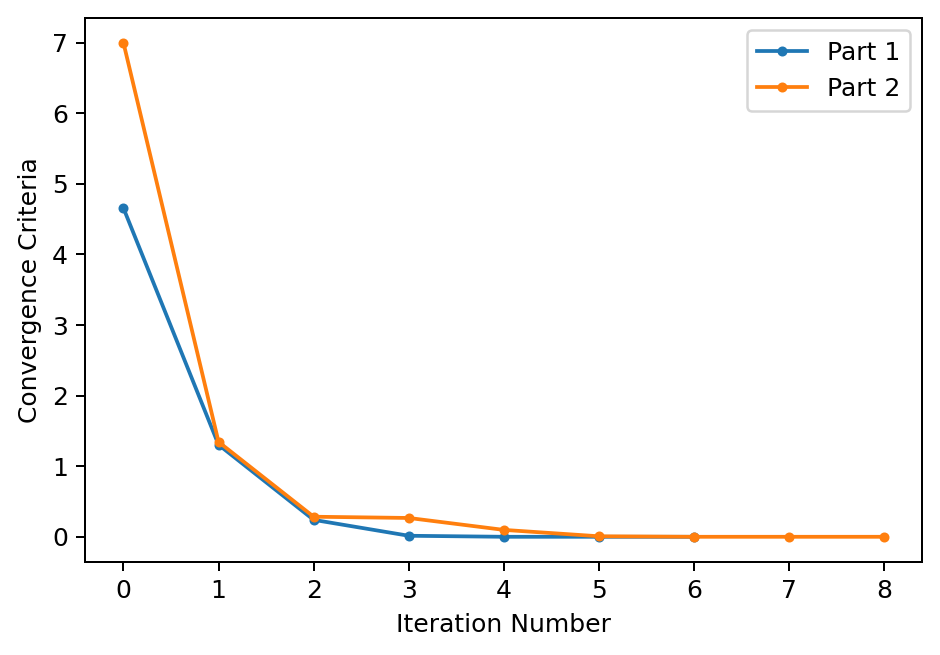
\includegraphics[width=4.5in]{HW2Figs/HW2P1.png}
	\caption{The general trend should look like this, all solutions converge to zero.}
    \centering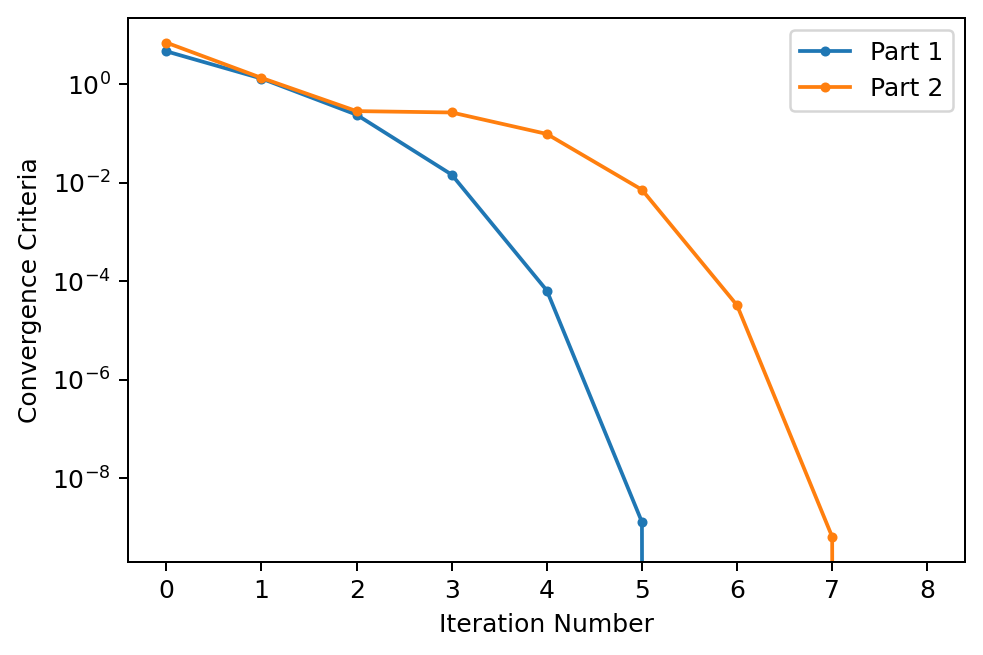
\includegraphics[width=4.5in]{HW2Figs/HW2P1b.png}
	\caption{If they plot on a log scale it should follow a trend similar to this}
	\label{fig:linearMethods}
\end{figure}

\color{black}
\fi

%%%%%%%%%%%%%%%%%%%%%%%%%%%%%%%%%%%%%%%%%%%%%%%%%%%%%%%%%%%%%%
\item[2. Gaussian Elimination (15 pts) By-hand.] Use Gaussian Elimination with scaled partial pivoting to solve the following system of equations:
    \begin{equation*}
    \begin{cases}
    \begin{aligned}
    x_1 + 3x_2 + x_3 &= -1 \\ 
    2x_1 + 2x_2 - 6x_3 &= 2 \\ 
    3x_1 - x_2 + 2x_3 &= 3
    \end{aligned}
    \end{cases}
    \end{equation*}

    \ifsolution
    \color{red}
        {\bf Solution:}\\
        The system is first expressed as an augmented matrix:
        \begin{equation*}
        \left[
          \begin{array}{cccc }
               2 & 1 & -1 & -2 \\
               4 & 1 &  2 &  4 \\
               6 & 1 &  1 & 6 \\
          \end{array}
        \right]
        \end{equation*}
        Forward elimination: First, we swap rows 1 and 3:
        \begin{equation*}
        \left[
          \begin{array}{cccc }
               6 & 1 &  1 & 6 \\
               4 & 1 &  2 &  4 \\
               2 & 1 &  -1 & -2 \\
          \end{array}
        \right]
        \end{equation*}
        Multiply row 1 by 1/2 and subtract from row 2. Multiply row 1 by 1/3 and subtract from row 3.
        \begin{equation*}
        \left[
          \begin{array}{cccc }
               6 & 1 &  1 & 6 \\
               0 & 1/3 &  4/3 &  0 \\
               0 & 2/3 &  -4/3 & -4 \\
          \end{array}
        \right]
        \end{equation*}
        Swap rows 2 and 3:
        \begin{equation*}
        \left[
          \begin{array}{cccc }
               6 & 1 &  1 & 6 \\
               0 & 2/3 &  -4/3 & -4 \\
               0 & 1/3 &  4/3 &  0 \\
          \end{array}
        \right]
        \end{equation*}
        Multiply row 2 by 1/2 and subtract from row 3.
        \begin{equation*}
        \left[
          \begin{array}{cccc }
               6 & 1 &  1 & 6 \\
               0 & 2/3 &  -4/3 & -4 \\
               0 & 0 &  2 &  2 \\
          \end{array}
        \right]
        \end{equation*}
        Back substitution:
        \begin{equation*}
        \begin{split}
         & x_3 = \dfrac{2}{2} = 1 \\
         & x_2 = \dfrac{3}{2} \left(-4+4/3 \right)=-4 \\
         & x_1 = \dfrac{1}{6} (6-1+4) = 1.5
        \end{split}
        \end{equation*}
    \color{black}
    \fi


%%%%%%%%%%%%%%%%%%%%%%%%%%%%%%%%%%%%%%%%%%%%%%%%%%%%%%%%%%%%%%
\item[3. An Aerospace Application (15 pts) Code.] The following question brings together elements from multiple methods we've covered so far. An Airbus A320 is flying at Mach 0.7. It's Pitot tubes, shown in Figure \ref{fig:Pitot},  measure the total, or stagnation, pressure (pressure when the air hits and is stopped by the tube) as well as the static free-stream pressure.

\begin{figure}[h!]
	\centering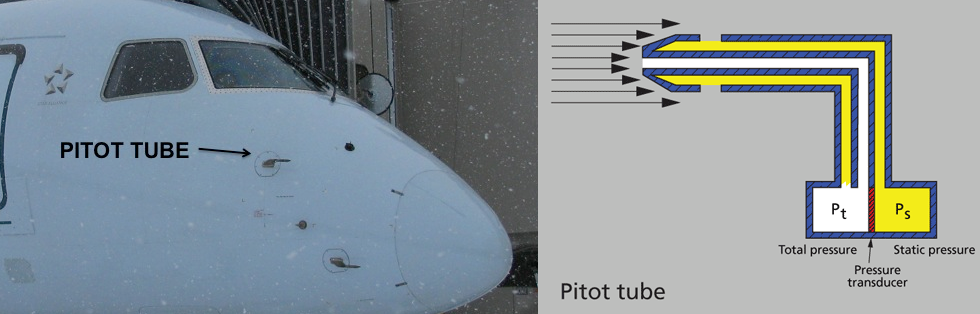
\includegraphics[width=4.5in]{HW2Figs/pitot}
	\caption{Pitot-Static Tubes: Used to measure the ratio of total pressure to static pressure for determining aircraft airspeed.}
	\label{fig:Pitot}
\end{figure}

The ratio of total to static pressure is determined to be: $p_0/p = 1.289$. The following equation relates this change in pressure to the inlet Mach number, $M$, and $\gamma$, the heat capacity ratio:

\begin{equation*}
\frac{p_0}{p}= \left[ 1 + \frac{\gamma-1}{2}M^2 \right]^{\gamma/(\gamma-1)}
\end{equation*}

Based on the given pressure ratio and Mach number, determine the value of $\gamma$ that satisfies this equation to \emph{four significant figures} of accuracy. State what method you used, how many iterations it took and give your final solution estimate. \textbf{Hint:} Don't try to solve analytically for $\gamma$. It might be helpful to plot the function $f(\gamma)$ over a range of values to help you pick a good initial first guess. Choose from any of the iterative methods learned in class to solve.

\ifsolution
\color{red}
\textbf{Solutions:}
\begin{enumerate} [label=(\alph*)]
	\item 	
	First, rearrange the equation so that it equates to zero:
	\begin{equation*}
	f(k) = 0 = \left[ 1 + \frac{\gamma-1}{2}M^2 \right]^{\gamma/(\gamma-1)} - \frac{p_0}{p}
	\end{equation*}
	
	A few different methods are possible to find the root. Taking the derivative of this function with respect to $\gamma$ is complicated and so Newton's Method is not recommended, so one can try the Secant Method. I ended up using the bisection method to estimate my solution.
	
%	\begin{figure}[ht]
%		\centering\includegraphics[scale=0.5]{HW2Figs/AERO222_HW2_P3.png}
%		\caption{In order to establish the initial bracket, plot the function to see roughly where it crosses the x-axis}
%		\label{fig:PitotPlot}
%    \end{figure}
	
	Error Tolerance: $\varepsilon = 1 \times 10^{-5}$ \\
	Initial Steps: $x_{0} = 0, \ x_{1} = 0.1$ \\
	Given Parameters: $M = 0.7, \ p_0/p = 1.289$ \\
	
	\textbf{Results from Secant Method:}
	
	Number of Iterations = 3
	
	$x_{Newton = 0.96498$
	
	$f(x_{Secant}) = -2.7110 \times 10^{-9}$
\end{enumerate}
\color{black}
\fi

%%%%%%%%%%%%%%%%%%%%%%%%%%%%%%%%%%%%%%%%%%%%%%%%%%%%%%%%%%%%%%
\item[4. Fixed Point Iteration and Range of Convergence (10 pts) By-hand.] A fixed point is a point where $x = g (x)$. We will use fixed point iteration to find these points and then apply concepts from fixed point iteration in order to determine the range of convergence for root solving methods.
\begin{enumerate} [label=(\alph*)]
	\item Given $x^2 -4x = 6x + 1$ give two functions, $g_1 (x)$ and $g_2 (x)$, for which we can perform fixed point iteration to solve for the roots of the equation above.
	\item Compute and draw the range of convergence (if any) on the interval $[-3,3]$ for both functions, $g_1 (x)$ and $g_2 (x)$.
\end{enumerate}
	
\ifsolution
\color{red}
{\bf Solution:}\\
\begin{figure}[ht]
	\centering\includegraphics[scale=0.45]{HW2Figs/HW12P2ab.png}
\label{fig:5ab}
\end{figure}
\color{black}
\fi
	

%%%%%%%%%%%%%%%%%%%%%%%%%%%%%%%%%%%%%%%%%%%%%%%%%%%%%%%%%%%%%%
\item[5. Newton's Method (20 pts) Code.] Given the function $f(x): -x^4 + 2x^3 = e^{-x} - 1$,
	\begin{enumerate} [label=(\alph*)]
		\item Find the root using Newton's method. Use $x_0 = 1.6$ and perform 5 iterations after the initial guess. Save the $x_k$ from each iteration to a vector.
		\item 	Determine if Newton's Method converges for the range of $x \in [-3,3]$ by using the convergence check for fixed point iteration. Provide a plot of $|g'(x)|$ to determine the range of convergence.
		\item Use the results from your code to provide a table of the estimated $x_k$ values from your Newton method iterations. Compute the order of convergence ($\alpha$) and the asymptotic error constant ($\lambda$) as accurately as possible using the $x_k$ values you have saved.
	\end{enumerate}

\ifsolution
\color{red}
        {\bf Solution:}\\
        \begin{enumerate} [label=(\alph*)]
        	
        	\item Applying the Newton Method, we obtain: \\
        	\begin{equation*}
        	\begin{cases}
        	    f(x) = -2x^3 + x - e^{-x} - 1 \\
        		f'(x) = -6x^2 + 1 + e^{-x} \\
        	    x_{n+1} = x_k-\dfrac{f(x_k)}{f'(x_k)} \\
     		    x_k = [-2.0000, -1.6406, -1.5372, -1.5283, -1.5282, -1.5282]
     		\end{cases}
     		\end{equation*}
        		\\
        	
        		
	        \item Newton's Method converges when $x_{n+1} = x_k$ for $n \rightarrow \infty$. Therefore, if fixed point iteration converges when applied to Newton's Method, then Newton's Method must also converge.  Writing Newton's Method in the recursive form:
	        \begin{equation*}
	        	x_{fpi} = g(x_{fpi}) = x_{fpi}-\frac{f(x_{fpi})}{f'(x_{fpi})}
	        \end{equation*}
	        	
	        Fixed point iteration converges for the interval $[a,b]$ if $|g'(x)| < 1$ for $x \in [a,b]$.
	        	
	        \begin{equation*}
	        	|g'(x)| = \left| \frac{f(x)f''(x)}{(f'(x))^2} \right|
	        \end{equation*}
	        	
	        $f(x) = -2x^3 + x - e^{-x} - 1$ \\
	        $f'(x) = -6x^2 + 1 + e^{-x}$ \\
	        $f''(x) = -12x - e^{-x}$ \\
	        	
	        Plugging this equation into Python and plotting, we can see that $\exists x \in [-3,3], \; |g'(x)| > 1 \implies$ FPI and the Newton Method are not guaranteed to converge on the interval [-3,3].
	        	
	        \begin{figure}[ht]	\centering\includegraphics[scale=0.7]{HW2Figs/AERO222_HW2_P5.png}
	        	\caption{$\left|g'(x)\right|$ for $x \in \left[-3,3\right]$}
	        \end{figure}
	
	        \item The order of convergence and asymptotic error constant can be approximated as:
   	
   	        \begin{equation*}
   	             \alpha= \frac{\ln e_{5}-\ln e_4}{\ln e_4 - \ln e_{3}} = 1.9977
   	        \end{equation*}
   	         \begin{equation*}
   	                     \lambda= \dfrac{e_5}{e_{4}^\alpha} = 0.7989
   	        \end{equation*}
		
\end{enumerate}
\color{black}
\fi

%%%%%%%%%%%%%%%%%%%%%%%%%%%%%%%%%%%%%%%%%%%%%%%%%%%%%%%%%%%%%%
\item[6. Matrix Operations (15 pts) Code.] Given the linear system,
\begin{equation*}
        A \, \B{x} = \begin{bmatrix*}[r] 3 & 2 & 7 & -1 & 4 \\ 6 & -2 & 0 & 2 & -2 \\ 4 & 1 & -1 & 2 & 4 \\ 2 & 10 & -6 & -4 & 1 \\ 5 & 3 & -1 & -8 & 3\end{bmatrix*} \begin{Bmatrix*} x_1\\ x_2\ \\ x_3\\ x_4\\ x_5\end{Bmatrix*} = \begin{Bmatrix*}[r] -1\\  3\\ 5\\ -6\\ 3\end{Bmatrix*} = \B{b}
    \end{equation*}
    Develop a code to:
    \begin{enumerate}[label=(\textbf{\alph*})]
        \item Perform the $L U$ Decomposition of $A$, and compare to 
        \verb|scipy.linalg.lu(A)|.
        \item Compute $A^{-1}$ using the Gauss-Jordan Method, and compare to 
        \verb|numpy.linalg.inv(A)|.
        \item Provide the solution of the system $A \, \B{x} = \B{b}$ using either $LU$ Decomposition {\bf{or}} the Gauss-Jordan Method.
    \end{enumerate}
    
\ifsolution
\color{red}
 {\bf Solution:}  \\
   \begin{enumerate}[label=(\textbf{\alph*})]
    \item
        \begin{equation*}
        P=
        \left[
          \begin{array}{ccccc}
      		 0        &      0       &       0   &      1       &       0   \\
     		 0        &      0       &       0   &      0       &       1   \\
     		  1        &      0       &       0   &      0       &       0   \\
     		  0        &      0       &       1   &      0       &       0   \\
     		  0        &      1       &       0   &      0       &       0   \\

          \end{array}
        \right]
        \end{equation*}\\
        \begin{equation*}
        L=
        \left[
                  \begin{array}{ccccc}
      		 1        &      0       &       0   &      0       &       0   \\
     		 -1        &      1       &       0   &      0       &       0   \\
     		  -0.5556        &      0.7704       &       1   &      0       &       0   \\
     		  -0.2222        &      0.2148       &       0.00077   &      1       &       0   \\
     		  -0.8889        &      0.3259       &       0.1121   &      -0.2159       &       1   \\
          \end{array}
        \right]
		 \end{equation*}\\
        \begin{equation*}
        U=
        \left[
                        \begin{array}{ccccc}
      		 -9        &      10       &       1   &      -4       &       6   \\
     		 0        &      15      &       -4   &      -12       &       10   \\
     		  0        &      0       &       10.6370   &      12.0222       &       -5.3704   \\
     		  0        &      0       &       0   &      4.5968       &       5.2263   \\
     		  0        &      0       &       0   &      0       &       0.8044   \\
          \end{array}
        \right]
                \end{equation*}

    \item
    \begin{equation*}
    A^{-1}=
        \left[
                        \begin{array}{ccccc}
      		 -0.0171        &      0.1863       &       0.0367   &      0.0644      &       -0.0077  \\
     		 0.1797        &      -1.3661      &       -0.1864   &      -0.7424      &       0.4136   \\
     		  -0.1573        &      2.2250       &       0.2345   &      1.2881       &       -0.6544  \\
     		  0.1591        &      -1.4134       &       -0.0876   &      -0.8305       &       0.3569   \\
     		  -0.1414        &      1.2431       &       0.2684   &      0.7322       &       -0.3539   \\
          \end{array}
        \right]
    \end{equation*}
    \item
     \begin{equation*}
    x =
    \left[
          \begin{array}{ccccc}
               1.5484 & -15.2508 & 24.9680 & -15.9077 &   14.4742 \\
          \end{array}
        \right] 
    \end{equation*}
    \end{enumerate}
       
    
\color{black}
\fi

\item[7. Jacobi Iterative Method (10 pts) Code.] Starting with the linear system given in Problem 2, transform the problem in the system, $A^* \B{x} = \B{b}$, by making $A^*$ be a diagonal dominant matrix ($|A^*(i, i)| \ge \sum_{k = 1}^5 \| A(i, k) \|$. Solve the obtained system using the Jacobi method,
    \begin{equation*}
        \B{x}_{k + 1} = D^{-1} \, \B{b} - D^{-1} \, O \, \B{x}_k
    \end{equation*}
    Stop iterating when the 2-norm of $|| \B{x}_{k + 1} -  \B{x}_k ||_2 / || \B{x}_{k + 1} ||_2$ is less than $10^{-12}$.
    \begin{enumerate} [label=(\alph*)]
	\item Print out the final values for $\B{x}_k$, the corresponding 2-norm of the error, and the number of iterations required.
	\item Repeat this exercise with the original matrix, $A$, and report the number of iterations required. Describe what has changed.
\end{enumerate}
    
    \ifsolution
    \color{red}
    {\bf Solutions}
    \begin{enumerate} [label=(\alph*)]
    \item
    \begin{equation*}
        x_k = \begin{Bmatrix*}[r] -0.3000\\ 0.4697\\ 0.1587\\ 0.0510\\ -0.0144\end{Bmatrix*}
    \end{equation*}
    2-norm of error: $\varepsilon = 6.4674 \cdot 10^{-7}$. Number of iterations: $k = 22$.\\
    \item
    \begin{equation*}
        x_k = \begin{Bmatrix*}[r] 2.0351\\ 2.3689\\ -7.2781\\ -1.9688\\ -inf\end{Bmatrix*}\times 10^{307}
    \end{equation*}
    2-norm of error: $\varepsilon = NaN $. Number of iterations: $k = 504$.
    \end{enumerate}
    \color{black}
    \fi

\end{description}
\end{document}